\section{L-TAE}
%The increasing accessibility and precision of Earth observation satellite data offers considerable opportunities for industrial and state actors alike. 
%This calls however for efficient methods able to process time-series on a global scale.
The paper ``Lightweight Temporal Self-Attention for Classifying Satellite Image Time Series" \cite{LTAE} was written by Vivien Sainte Fare Garnot, and Loic Landrieu, and published in 2020.

The authors introduce a new deep learning model for classifying satellite image time series, which utilizes a modified version of the Temporal Attention Encoder.

In their proposed network, the channels of the temporal inputs are distributed among several attention heads that operate in parallel. These heads extract specialized temporal features, which are then concatenated into a single representation. The authors show that their approach achieves superior performance compared to other state-of-the-art time series classification algorithms on an open-access satellite image dataset, while using significantly fewer parameters and reduced computational complexity.

Overall, the paper presents a novel method for classifying satellite image time series, utilizing a lightweight variant of temporal self-attention and outperforming other state-of-the-art approaches.

\subsection{Multi-Headed Self-Attention}

The original version of self-attention, which was initially developed for text translation as described in \cite{vaswani}, involves three main steps.
Firstly, for each position "t" in the input sequence, a triplet of key-query-value is computed, denoted as $k^{(t)}$, $q^{(t)}$, and $v^{(t)}$, respectively, by applying a shared linear layer to the input $e^{(t)}$.
Secondly, attention masks are calculated, representing the compatibility (dot-product) between the queries and the keys of previous elements in the sequence. 
Lastly, an output is assigned to each position in the sequence, which is the sum of previous values weighted by the corresponding attention mask.

To enable each head to specialize in detecting certain characteristics of the feature vectors, the self-attention process is performed in parallel for "H" sets of independent parameters or heads, and the outputs are concatenated.
This approach is used by Rußwurm et al. \cite{russwurm2019self} to embed sequences of satellite observations by max-pooling the resulting sequence of outputs in the temporal dimension.

Garnot et al. \cite{garnot2020satellite} introduce a modified self-attention scheme called the Temporal Attention Encoder (TAE).
Firstly, they propose using the input embeddings as values (i.e., $v^{(t)} = e^{(t)}$) directly, which takes advantage of the end-to-end training of the image embedding functions along with the TAE.
They also define a single master query $\hat{q}$ for each sequence, which is computed from the temporal average of the queries.
The master query is compared to the sequence of keys to produce a single attention mask of dimension $T$, which is used to weight the temporal mean of values into a single feature vector.



\subsection{Model}
Their work is an extension of previous efforts in adapting multi-headed self-attention for sequence embedding.
The primary objective is to optimize efficiency, specifically with regards to parameter count and computational load.

\begin{figure}[!htbp]
  \centering
  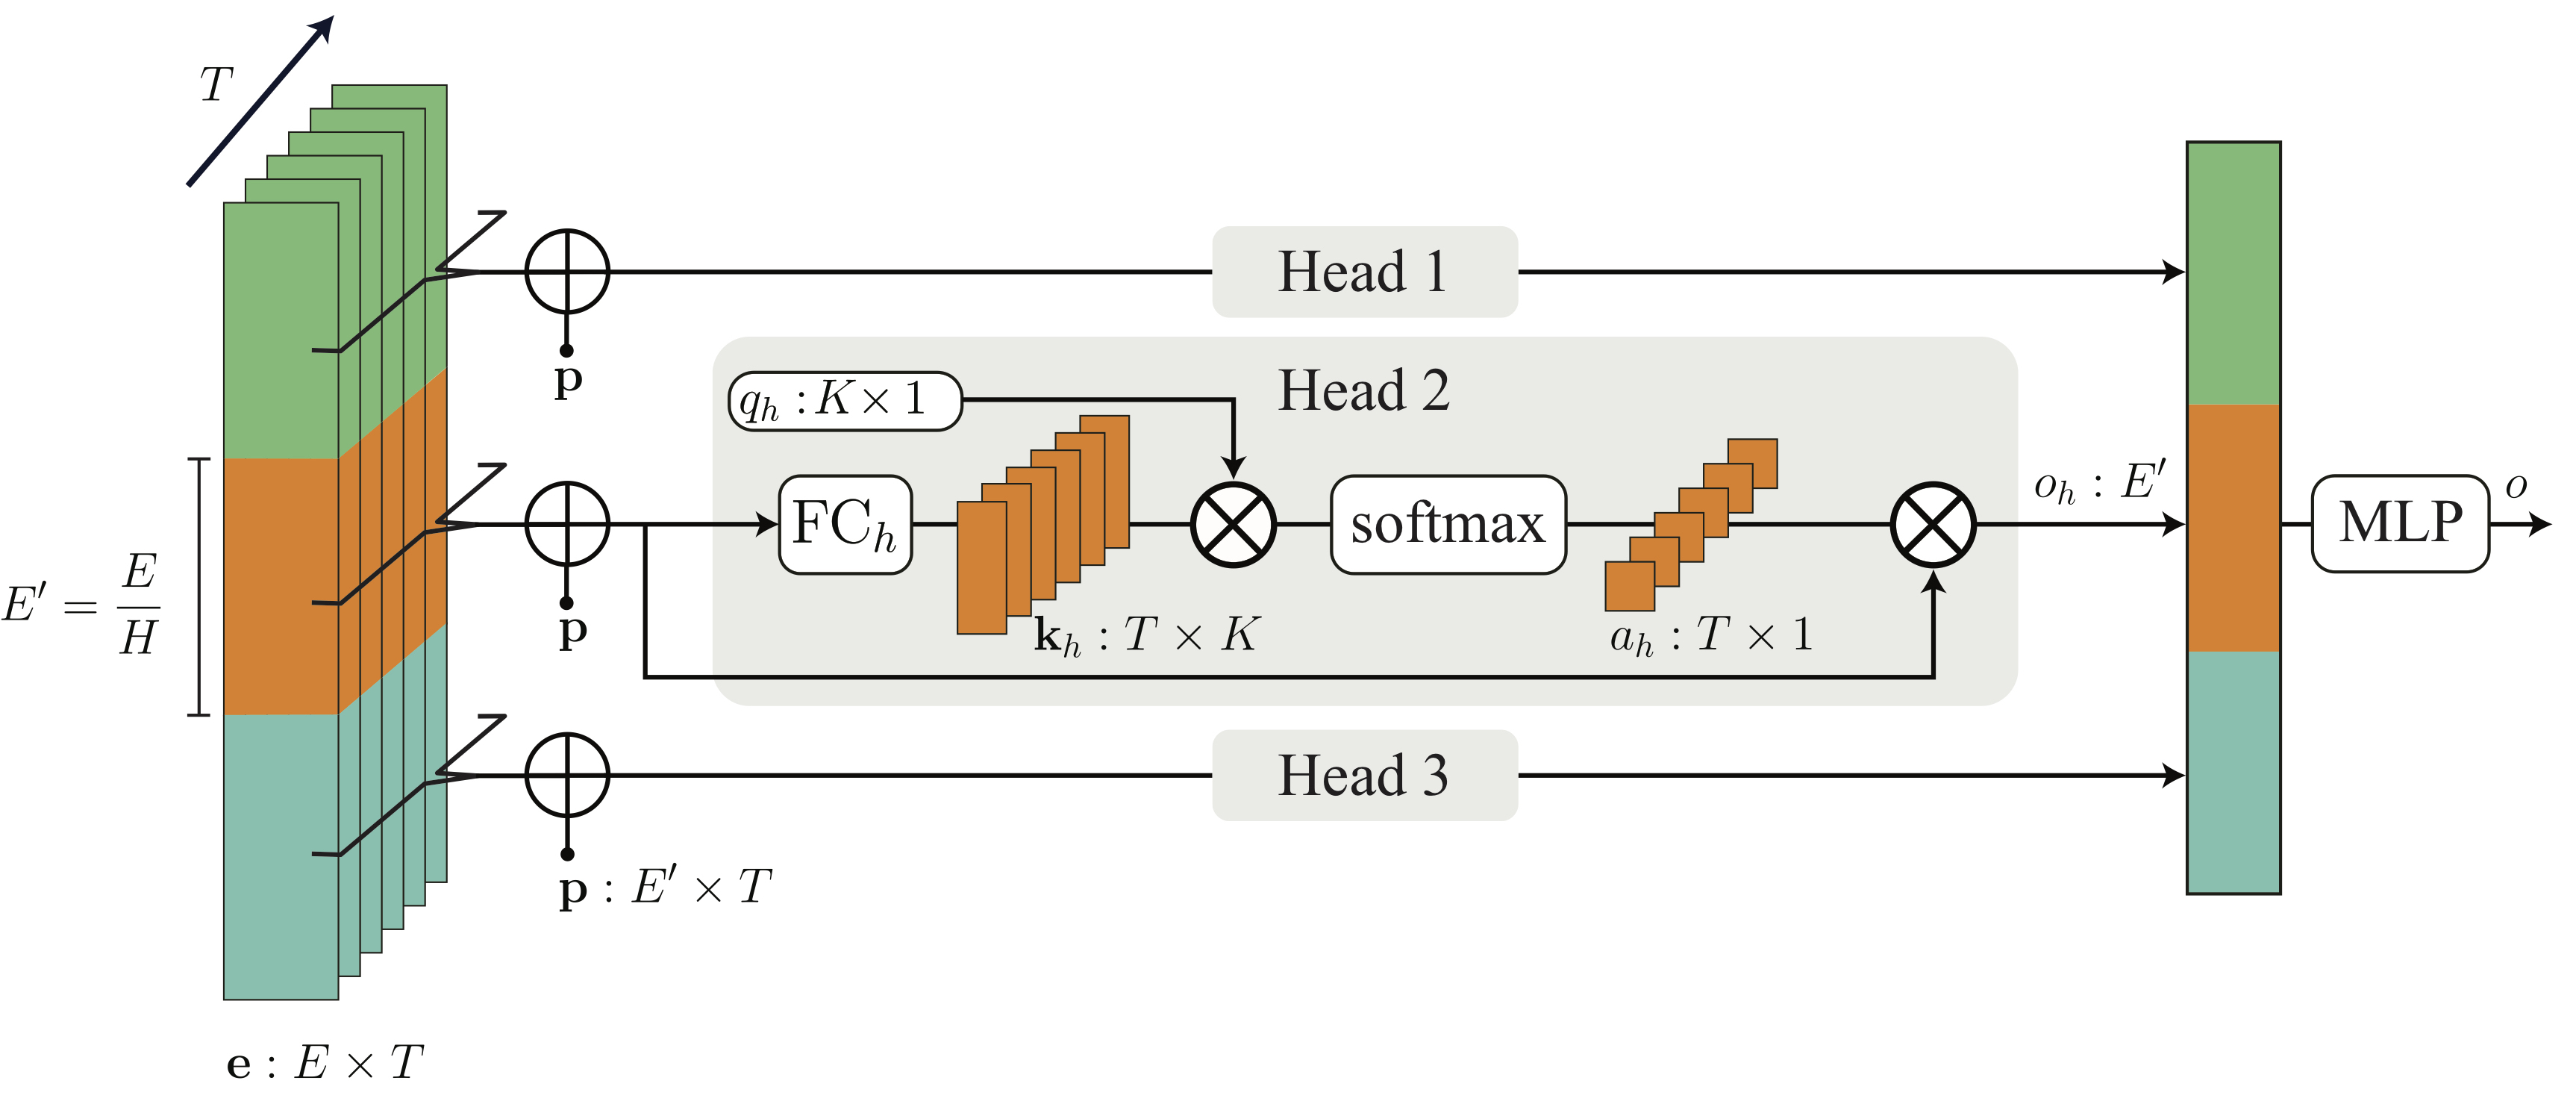
\includegraphics[width=1\textwidth]{LTAE}
  \caption{Light Temporal Attention Encoder  (L-TAE) module processing an input sequence e of $T$ vectors of
  size $E$, with $H = 3$ heads and keys of size $K$. The channels of the input embeddings
  are distributed among heads. Each head uses a learnt query $\hat{q_h}$, while a linear layer
  $FC_h$ maps inputs to keys. The outputs of all heads are concatenated into a vector with
  the same size as the input embeddings, regardless of the number of heads \cite{LTAE}}
  \label{fig:LTAErchitecture}
\end{figure}

\begin{paragraph}{Channel Grouping} 
The proposal is to divide the $E$ channels of the input elements into $H$ groups of size $E' = E/H$ following the approach of Wu et al. \cite{wu2018group}, where $H$ refers to the number of heads. The groups of input channels for the $h$-th group of the t-th element of the input sequence (\ref{eq:LTAE1}) are denoted by $e^{(t)}_h$.

To encode the number of days elapsed since the beginning of the sequence, an $E'$-dimensional positional vector $p$ with a characteristic scale $\tau = 1000$ is used (\ref{eq:LTAE2}).
To enable each head to access this information, the vector $p$ is replicated and added to every channel group.
This approach allows each head to work in parallel on its corresponding group of channels, reducing the computational expense of calculating keys and queries. Additionally, it allows each head to specialize alongside its channel group and avoid redundant operations between heads.
\end{paragraph} 

\begin{paragraph}{Query-as-Parameter} 
The K-dimensional master query $q_h$ of each head $h$ is defined as a model parameter instead of the results of a linear layer.
This approach has the immediate advantage of reducing the number of parameters required.
Although this method lacks flexibility, it is compensated by the greater number of heads available.
\end{paragraph} 

\begin{paragraph}{Attention Masks}
The approach involves using a learned linear layer (\ref{eq:LTAE3}) solely for obtaining the keys, bypassing the values $(v^{(t)} = e^{(t)})$, and employing model parameters for the queries.
For each head $h$, the attention masks $a_h \in [0, 1]^T$ are obtained by scaling the softmax of the dot product between the keys and the master query (\ref{eq:LTAE4}).
The outputs $o_h$ of each head are determined by summing the corresponding inputs weighted by the attention mask $a_h$ along the temporal dimension (\ref{eq:LTAE5}).
Following this step, the outputs of each head are concatenated to form a vector of size $E$, which is then processed through a multi-layer perceptron MLP to achieve the desired size (\ref{eq:LTAE6}).

A schematic representation of the network is provided in Figure \ref{fig:LTAErchitecture}.
In summary, the various steps of the L-TAE method can be summarized by the following operations for $h = 1...H$ and $t = 1...T$:

\begin{align}
  e^{(t)}_h &= e^{(t)}[(h-1) E'...hE']                                  \label{eq:LTAE1}\\
  [p^{(t)}] &= sin(day(t)/\tau^{\frac{i}{E'}})                          \label{eq:LTAE2}\\
  k^{(t)}_h &= FC_h(e^{(t)}_h + p^{(t)})                                \label{eq:LTAE3}\\
  a_h       &= softmax \Bigr(\frac{1}{\sqrt{K}} \Bigr[[q_h \cdot k^{(t)}_h\Bigr]^T_{t=1}\Bigr) \label{eq:LTAE4}\\
  o_h       &= \sum_{t=1}^{T} a_h[t] (e^{(t)}_h + p^{(t)})              \label{eq:LTAE5}\\
  o         &= MLP([o_1,...,o_H]).                                      \label{eq:LTAE6}
\end{align}

\end{paragraph}

\begin{paragraph}{ Spatio-temporal classifier}
The L-TAE temporal encoder is designed to be trained together with a spatial encoding module and a decoder module in an end-to-end manner (\ref{eq:LTAE7}).
  
The spatial encoder $S$ is responsible for mapping a sequence of raw inputs $X^{(t)}$ to a sequence of learned features $e^{(t)}$, computed independently at each position of the sequence.
On the other hand, the decoder $D$ is responsible for mapping the output $o$ of the L-TAE to a target vector $y$, which can be class logits in the case of a classification task.
\end{paragraph}

\begin{equation}
  \label{eq:LTAE7}
  \Bigr[X^{(t)}\Bigr]^T_{t=1} \quad \xrightarrow{S} \quad \Bigr[e^{(t)}\Bigr]^T_{t=1} \quad \xrightarrow{L\mbox{--}TAE} \quad o \quad \xrightarrow{D} \quad y
\end{equation}


\subsection{Data preparation}
%- splits\\

As described in Section \ref{sec:tempCNNDataPreparation}, we partitioned the dataset into three subsets: training (60\%), validation (20\%), and test (20\%). 
To ensure that each set had a similar class distribution and to avoid spatial autocorrelation, we took necessary precautions.

The implementation of the model was carried out using PyTorch framework. For the purpose of embedding input images, the Pixel Set Encoder (PSE) was utilized, which has previously been shown to be a suitable technique for satellite image datasets \cite{garnot2020satellite}.

While the PSE method worked well for the original dataset, we developed a new encoder called Dense Encoder (DE) that better suited the needs of our dataset.
The DE is a simple linear neural network that takes a 16-channel image as input and produces a 64-dimensional vector using a hyperbolic tangent (tanh) activation function. 
The DE was designed to be computationally efficient, allowing for faster training and inference times, while still maintaining strong performance on our specific dataset.

% - dates\\
% - pytorch implementation\\
% - PixelSetEncoder\\
% - DenseEncoder\\
% -- tanh

\subsection{Experimental results}

After adapting the L-TAE model to our dataset, we trained it by adjusting the hyper-parameters to find the optimal configuration, guided by the results of their research.

\begin{table}[ht]
  \centering
  \begin{tabular}{l p{12cm}}   
     Param & Description \\[0.2cm] 
     \hline \\[-0.2cm]  
     E & size of the embeddings ($E$), if input vectors are of a different size, a linear layer is used to project them d\_model-dimensional space \\
     H & Number of attention heads  \\
     K & Dimension of the key and query vectors  \\
     MLP & Number of neurons in the layers of MLP \\
  \end{tabular}
  \caption{Hyper-parameters of L-TAE model}
  \label{tab:LTAEconfig}
\end{table}

In the following, we have described the findings of the authors on the impact of the different hyperparameters on the performance of the model.

\begin{paragraph} {Number of heads} 
It appears that the performance is only marginally impacted by the number of heads. 
Their hypothesis is that an increase in the number of heads ($H$) can be advantageous, but a reduction in group size ($E'$) can be detrimental.
\end{paragraph}

\begin{paragraph} {Dimension of keys}
The experiments indicate that smaller key dimensions, as opposed to the typical values used in NLP or for the TAE ($K = 32$), lead to better performance on the problem.
The L-TAE can achieve comparable performance to the TAE with only 2-dimensional keys.
\end{paragraph}

\begin{paragraph} {Dimension of Input}
The expected outcome of having larger input embeddings is an increase in performance, as it corresponds to a more comprehensive representation.
Nevertheless, on the dataset being considered, the benefits of increasing the number of parameters are diminishing.
\end{paragraph}

\begin{paragraph} {Query-as-Parameter}
To evaluate the impact of the design choices, a variation of the network is trained using the same master-query scheme as the TAE.
The larger linear layer that results increases the model's size to a total of 170k parameters.
The observation that the resulting mIoU is only 49.7 suggests that the query-as-parameter scheme is advantageous not only in terms of compactness but also for achieving better performance.
\end{paragraph}

Table \ref{tab:LTAEresults} presents the performance results of the L-TAE architecture with different configurations of the following hyper-parameters: number of heads H, dimension of keys K, and number of channels E in the input sequence.
All the results were obtained through a 4-fold cross-validation scheme.
The performance metrics were measured for two different scenarios: one where missing values were imputed and one where missing values were not imputed.

\begin{table}[ht]
  \centering
  \begin{tabular}{cccclrr} 
     Params & E & H & K & MLP & No imputation & Pre imputation\\[0.2cm] 
     \hline \\[-0.2cm] 
     43k & 	128 & 	8 & 	8 & 	128 & 	$93.37 \pm 1.65$ & 	$93.08 \pm 1.16$\\ 
     68k & 	128 & 	16 & 	8 & 	128 - 128 & 	$93.43 \pm 1.37$ & 	$93.39 \pm 1.16$\\ 
     123k & 	256 & 	16 & 	8 & 	256 - 128 & 	$93.15 \pm 1.72$ & 	$93.44 \pm 1.22$\\ 
     299k & 	512 & 	32 & 	8 & 	512 - 128 & 	$\mathbf{93.65 \pm 1.30}$ & 	$93.40 \pm 1.16$\\ 
     749k & 	1024 & 	32 & 	8 & 	1024 - 256 - 128 & 	$92.91 \pm 1.90$ & 	$\mathbf{93.58 \pm 1.29}$\\ 
  \end{tabular}
  \caption{Results of the L-TAE model with different parameters}
  \label{tab:LTAEresults}
\end{table}

Overall, the results reported in Table \ref{tab:LTAEresults} demonstrate the effectiveness of the L-TAE architecture in accurately classifying the input data even with a lower number of parameters. 
The inclusion of missing data through imputation did not significantly impact the performance of the model, suggesting that the L-TAE architecture is robust to the presence of missing values.